\textbf{{1. PPP协议的组成}}

\textbf{a.~}一个将IP数据报封装到串行链路的方法;

\textbf{b.~}一个链路控制协议(LCP),用于建立、配置和测试数据链路连接,并在不需要时将它们释放;

\textbf{c.~}一套网络控制协议(NCP),其中每个协议支持不同的网络层协议,用来建立和配置不同的网络层协议。

\textbf{{2.PPP协议的帧格式}}

PPP协议的帧格式如下图所示。

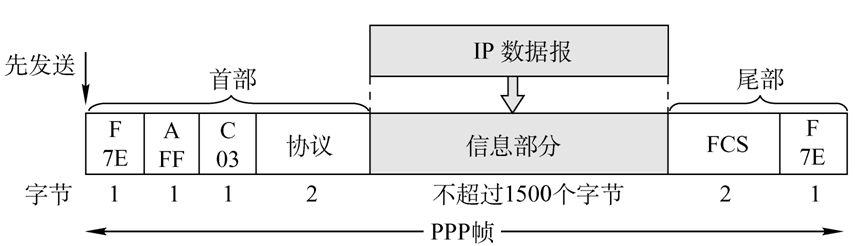
\includegraphics[width=3.12500in,height=0.89583in]{png-jpeg-pics/1E644CC65BB369A7E3A5DEDC1FCDD97C.png}

\textbf{1)标志字段(F)。}首部和尾部各占1个字节,规定为Ox7E。

\textbf{2)地址字段(A)。}占1个字节。规定为OxFF,没有为什么。

\textbf{3)控制字段(C)。}占1个字节。规定为Ox03,没有为什么。

\textbf{4)协议字段。}占2个字节。例如,当协议字段为
0x0021时,PPP帧的信息字段就是IP
数据报;若为0xC021,则信息字段是PPP链路控制数据;若为0x8021,则表示这是网络控制数据。

\textbf{5)信息部分。}占0~1500个字节。为什么不是46~1500个字节?因为PPP是点对点的,并不是总线型,所以无需采用CSMA/CD协议,自然就没有最短帧。另外,当数据部分出现和标志位一样的比特组合时,就需要采用一些措施来实现透明传输(上面的补充知识点已讲)。

\textbf{6)帧检验序列(FCS)。}占2个字节,即循环冗余码检验中的冗余码。检验区间包括地址字段、控制字段、协议字段和信息字段。

\textbf{{3.PPP的工作状态}}

{当用户拨号接入ISP时,路由器的调制解调器对拨号做出确认,{\textbf{并建立一条物理连接}}。这时,个人计算机向路由器发送一系列的LCP分组(封装成多个PPP帧)。这些分组及其响应选择了将要使用的一些PPP参数。接着就进行网络层配置,网络控制协议(NCP)给新接入的个人计算机分配一个临时的IP地址。这样,个人计算机就成为因特网上的一个主机了。}

{
当用户通信完毕时,NCP释放网络层连接,收回原来分配出去的IP地址。接着,LCP释放数据链路层连接,最后释放物理层连接。}

{\textbf{{4. 总结}}}

{{\textbf{a.~}PPP是一个\textbf{面向字节的协议}。}}

{\textbf{b.~}PPP不需要的功能:纠错(PPP只负责检错)、流量控制(由TCP负责)、序号(PPP是不可靠传输协议,所以不需要对帧进行编号)、多点线路(PPP是点对点的通信方式)、半双工或单工(PPP只支持全双工链路)。}
